\chapter{Overview}
\label{chp:overview}
\ProductName{} can run on a single Unix host or several co-operating machines.
The Windows software can manage the batch jobs on one or more of these
Unix hosts. It can also submit new jobs to any other host, with a default of one particular host, known as the
Server. The Server is specified at the PC, hence different PCs can use
different Servers and each PC can change Server.

The program which manages jobs is called \progname{btqw} and
the program to submit jobs is called \progname{btrw}. Their
relationship to a group of three Unix hosts might look like this:

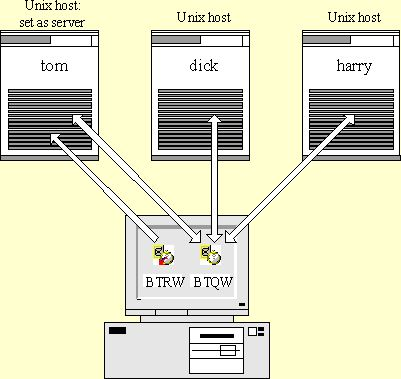
\includegraphics{img/win1.jpg} 

In this example, program \progname{btqw} can see and manage
jobs on hosts \exampletext{tom}, \exampletext{dick}
and \exampletext{harry}. Program \progname{btrw}
submits new jobs by default to host \exampletext{tom}.

\section{Jobs \& Variables}
\ProductName{} maintains a queue of batch jobs. Each batch job consists of a
script and a specification of what \ProductName{} should do with it.

Job Control Variables are provided by \ProductName{} to manage dependencies
between jobs. Jobs can include specifications to set or modify the
values of variables when they start or finish. On finishing, different
operations can be specified for variables depending on whether the job
worked or failed.

The job specification also includes conditions on variables, which
\ProductName{} tests before letting that job start.

\section{Owners, Groups and Modes}
Like Unix files, all jobs and variables are owned by a user and belong
to a particular group. This is used to say who may see and edit a job
or variable. These work with the protection modes.

Each job and variable is given a \textit{protection mode}. This consists
of a set of permissions dictating how various users may, or may not,
access the job or variable. The modes are like those on Unix files,
providing \textit{user}, \textit{group} and \textit{other} access. An
expanded set of permissions has been devised to enable the permissions
to control separate operations.

The modes of jobs and variables are set when they are created, however
users authorised by the mode may reset them subsequently.

In the case of \textit{jobs}, the modes set by
\progname{btrw} are used, in default of which a set of
default modes for the given user are set.

